\documentclass{beamer}
 
\usepackage[utf8]{inputenc}
\usepackage{wrapfig}
 
 
%Information to be included in the title page:
\title{BOX2D PROJECT}
\author{Rana Prathap  \hspace{5pt} Sreenivas \hspace{5pt}  Srinath  \\
        \hspace{15pt} 140050068 \hspace{5pt}     140050078 \hspace{5pt}   140050080\\
        }
\institute{IIT Bombay}
\date{\today}

\begin{document}
 
\frame{\titlepage}
 
\begin{frame}
\frametitle{Overview}
\begin{itemize}
\item<1-> Introduction
\item<1-> Elements
\item<1-> Joints
\end{itemize}
\end{frame}

\begin{frame}
\frametitle{Introduction}
 \vspace{-40pt}
We simulated a simple Rube Goldberg machine consisting of static and dynamic bodies
\begin{itemize}
 \item<1-> It is basically the movement of balls to finally kick the pin on the ground off
 \item<1-> This is achieved by the use of some elements and joints explained below
\end{itemize}
\end{frame}

\begin{frame}
 \frametitle{Elements}
 \vspace{-40pt}
  Elements implemented in our project include double pulley system, 
  \begin{wrapfigure}{r}{0.5\textwidth} 
   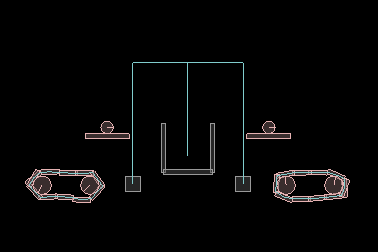
\includegraphics[width=0.2\textwidth]{doublepulley.png}\\
   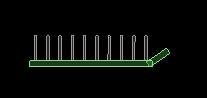
\includegraphics[width=0.2\textwidth]{dominos.png}
    \end{wrapfigure}
  conveyor belts, dominos, balls

\end{frame}

\begin{frame}
 \frametitle{Joints}
 \vspace{-40pt}
  The following are the various joints used in our project
  \begin{wrapfigure}{r}{0.5\textwidth} 
   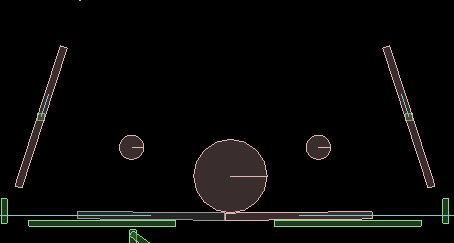
\includegraphics[width=0.2\textwidth]{rev.png}
    \end{wrapfigure}
  Revolute joints

\end{frame}
 
\end{document}